\documentclass[]{report}
\usepackage{graphicx}
\usepackage{url}
\usepackage{graphics}
\usepackage{rotating}
\usepackage{lscape}
\usepackage{listings}

% Title Page
\title{Distributed/Cluster Computing for Data  Stream Mining: Draft Notes}
\author{Vladimir Petko}

\begin{document}
\lstset{language=Java}   
\maketitle

\section*{Abstract}

The thesis is focused on elucidating GPU computing feasibility for clustering tasks

\section*{Introduction}

In real world applications such as industrial monitoring, sensor networks, financial data generate large unbounded streams of data which has to be processed with pre-defined response time. The processors capabilities limit the bandwidth of the stream which can be processed. Parallelizing processing algorithm will increase maximum bandwidth while maintaining the response time requirement.
\section*{Previous Work}
\subsection*{General Purpose GPU Computing Frameworks}

The tree of the GP-GPU technologies is presented in the Figure 1. 
\begin{figure}[htp]
	\resizebox{\textwidth}{!}{
		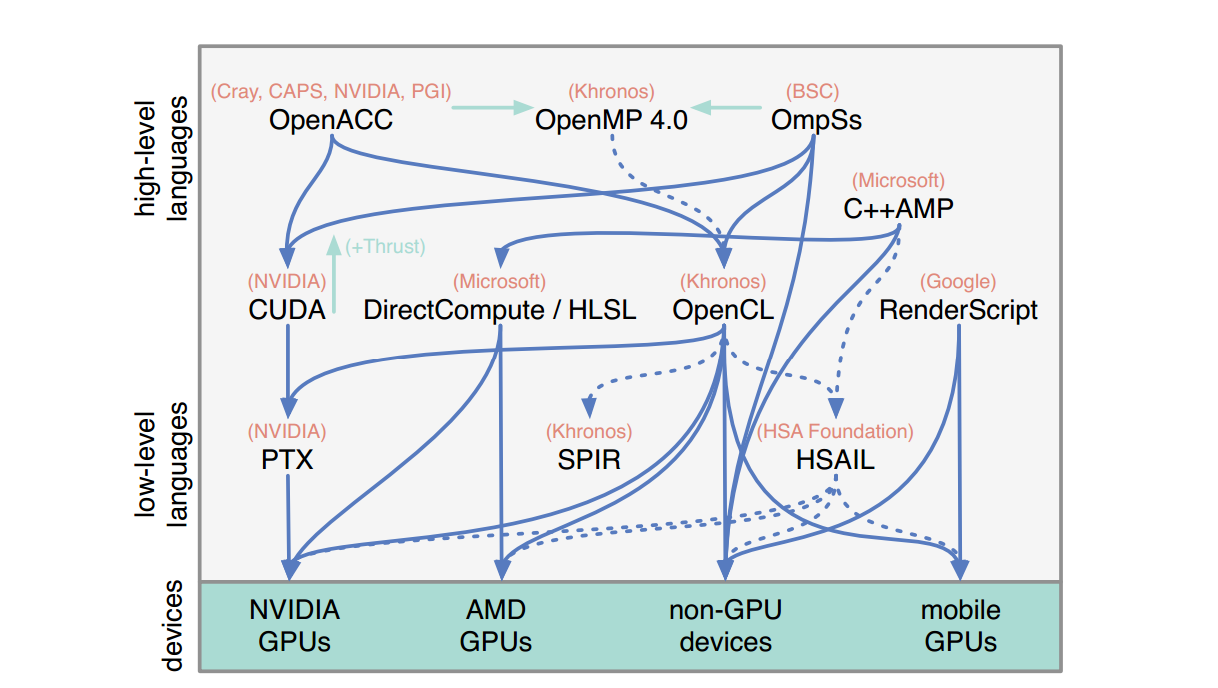
\includegraphics[width=\textwidth]{Figure1-GP-GPU-Frameworks.png}
		}
	\caption{\label{GpuTechTree} GP GPU technologies tree \cite{NugterenFig27}}
\end{figure}

\paragraph*{GPU-specific Languages}
 GPU-specific languages provide a programming model consistent with the GPU hardware implementation. 
 Modern GPUs implement SIMT (Single Instruction - Multple Thread) execution model (NB. AMD/NVIDIA desktop GPUs) 
 The memory on GPU is divided in 3 tiers 
\begin{itemize}
  	\item \textit{private/register} - private to the current thread
  	\item \textit{local} - shared within a \textit{threadblock}
  	\item \textit{global} - accessible by every thread
\end{itemize}
Each of the listed languages provides following abstractions:
 \begin{itemize}
 	\item \textit{Kernel} - a unit of execution
 	\item \textit{Thread} - a single unit of processed data 
 	\item \textit{Threadblock} - a group of \textit{threads} sharing same \textit{kernel} and \textit{local} memory.
 \end{itemize}

The unit of scheduling is called \textit{wavefront} in AMD terminology or \textit{warp} in NVIDIA and typically consists of 32 threads on NVIDIA and 64 on AMD hardware. The GPU chip is equipped with a number of SIMT cores which execute same instruction for each \textit{warp}. 
Divergence of control results in underload of the processing units and reduces performance. The branching should be reduced to wavefront granularity to avoid wasting execution cycles\cite{megakernel}(better citation?). Should be noted that the wavefront size is a hardware specific feature which should be specified at the runtime.
  
\begin{itemize}
\item CUDA - A programming language for NVIDIA hardware
\item OpenCL - Open standard from Khronos group
\item RenderScript - Android GPU computing component
\item DirectCompute/HLSL - Microsoft Parallel Computing.
\end{itemize}


\paragraph*{Low-Level Languages}
\begin{itemize}
\item PTX - NVIDA CUDA Assembly
\item SPIR - Standard Portable Intermediate Representation from Khronos group. OpenCL assembly.
\item HSAIL -  HSA Foundation assembly languange
\end{itemize}

\paragraph*{High Level Languages}

OpenACC and OpenMP are high level parallel programming frameworks that specify a set of annotations, environment variables and library routines for shared memory parallelism in C/C++ and Fortran programs\cite{OpenACC}\cite{OpenMP}.
Microsoft C++ AMP\cite{MSDN_AMP} is a C++ library which enables parallel computations for CPU and GPUs (using Microsoft DirectX Shading Language)
Rootbear GPU compiler provides a transparent compilation of Java code into CUDA\cite{Rootbear}.
Aparapi provides a way to generate OpenCL kernel code from Java, theoretically allowing code which can be executed on CPU and offloaded to GPU if needed\cite{Aparapi}.
Project Sumatra is a OpenJDK project which focuses on development of the Hotspot virtual machine capable of offloading JDK 8 Stream API\cite{StreamAPI} computations to the GPU\cite{Sumatra}.
\paragraph*{Limitations}
\subparagraph*{Input Size}
The massively parallel nature of GPU platforms require a certain amount of data to be passed to the kernel to achieve maximum performance. Table \ref{table:GlobalSize} shows execution time of a kernel which assigns index to each array element $ X_{i} = i $ on AMD A8-7600. The execution time starts to increase when input size is above 1024 and remains constant for lower values.
To maximum performance on AMD A8-7600 will be achieved when input size will exceed 1024 elements.
\begin{table}[htbp]

\begin{tabular}{|c|c|}
\hline 
Global Size & Execution Time ($\mu$sec) \\ 
\hline 
256 & 8 \\ 
\hline 
512 & 8 \\ 
\hline 
768 & 8 \\ 
\hline 
1024 & 8 \\ 
\hline 
1280 & 9 \\ 
\hline 
2560 & 9 \\ 
\hline 
2816 & 10 \\ 
\hline 
3072 & 10 \\
\hline 
3584 & 11 \\
\hline 
4608 & 11 \\
\hline 
4864 & 12 \\
\hline 
\end{tabular} 
\caption{Input Size and Execution Time}
\label{table:GlobalSize}   
\end{table}

\subparagraph*{GPU Memory Size and Host-GPU Transfer}
The discrete GPU requires transfer of data from the host to the GPU memory which adds additional overhead to the computations and requires task partitioning according to the memory specification of GPU\cite{Sismanis2012}. 
Memory transfer is a bottleneck for Aparapi and its developers allow explicit memory management\cite{Aparapi}. This effectively reduces framework which promises CPU-GPU interoperability to the Java wrapper of the OpenCL API.

\subparagraph*{Kernel Launch Time}
There is a constant time needed to setup kernel launch which might offset any gain from parallelization if the data can be processed sequentially faster.(NB. Amdahl's law)


\subsection*{HSA Platform}
Heterogeneous System Architecture plaftorm specifiction introduces a set of requirements that allow both GPUs and CPU share same memory space and synchronize execution\cite{HSAPlatform}. The introduction of shared memory addresses memory transfer limitation and allows to use all available host memory as a kernel input data. This makes HSA platform an interesting choice for the implementation of online algorithms as it is supposed to have lowest latency of all GP GPU frameworks.
\textit{Software Available}:
At the moment (Feb 2014) there is OpenCL->HSAIL compiler available\cite{CLOC} and a Linux-based runtime environment\cite{HSAGithub}. 

\paragraph*{HSA Memory Model}
\textit{TODO}
\paragraph*{HSA Queues}
Similiar to OpenCL\cite{OpenCL} HSA uses queues to schedule code execution. A HSA \textit{queue} is a ringbuffer which contains \textit{packets} with either call or synchronization parameters. The queue maintains two indexes - read index and write index. Write index is modified by the user and used to submit packets to the queue. The read index is updated by the packet processor whenever the packet is taken for execution. As soon as packet is written to the queue the ownership is taken by the HSA packet processor and it may change packet contents at any time\cite{HSAPlatform}.
\textit{TODO: Continue}
\paragraph*{HSA Signals}
HSA uses \textit{signals} to perform synchronization between host and kernels being executed or to signal completion of the task.
\textit{TODO: Continue}
\paragraph*{Implementation Notes}
Scenario: submit packet, wait for completion, submit another one yields 8 $\mu$sec per packet and submit $ N $ packets with a shared completion flag, wait for the completion flag become updated by $N$ results in 193 $\mu$sec per packet.
There is a constant time needed to setup kernel launch, e.g. for AMD A8-7600, it is 6 $\mu$sec using HSA. 


\subsection*{Machine Learning and General Purpose GPU Computing}
\subsubsection*{k-Nearest Neighbours}

k-Nearest Neighbours method is a non-parametric method used for the classification and regression. It computes a given instance distance to the examples with the known label and either provides a class membership for the classification which is a class most common among nearest neighbours or an object property value which is an average of the nearest neighbours. The error rate bound by the twice the Bayes error if the number of examples approaches infinity\cite{Cover:2006:NNP:2263261.2267456}.
The naive approach computes distance to each example and has computational complexity  $ O(N^{d}) $ where N - number of examples and d - cardinality of the example. \cite{something}
The method optimizations deal with organizing the search space to reduce number of distance calculations. Examples would be branch and bounds \cite{something} methods - [list trees],  and  approximate methods, e.g.  - Locality sensivity hash.\cite{something}
In relation to data stream classification there are two problems:
\begin{itemize}
\item Forward k-NN - for an given sliding window of examples find classification of the variable query
\item Reverse k-NN - for a given fixed query form a window of examples nearest to it. This approach is discussed in Efficiently Processing Continuous k-NN Queries on Data Streams\cite{BohmBeng}.
\end{itemize}

There is a number of implementations of the offline k-NN algorithm for GP-GPU: brute force approach\cite{AliDashti}\cite{Kuang_l}\cite{Kato}\cite{Sismanis2012}, kd-tree\cite{gieseke2014buffer}\cite{Zhou}, approximate \cite{flann_pami_2014}\cite{VLSH}. 
The brute force implementation consists of distance calculation and sorting phase. The distances to the query a computed as a vector-matrix multiplication or if several queries are processed at once as a matrix-matrix multiplication. GPU implementation of those routines is available as a part of cuBLAS library\cite{cuBLAS}. Sorting phase finds k nearest of all the computed distances\cite{Sismanis2012}. Sismanis et. al\cite{Sismanis2012} provide time complexity of reduced sort algorithms and evaluates their performance on GPU, proposes to interleave distance calculation and sorting phases to hide latency - the data for the distance calculation should be offloaded to GPU while it performs the sorting phase. The input data in the brute-force approach is partitioned according to the GPU memory capabilities and does not use examples's spatial information.
The kd-tree approach presented by Gieske et. al focuses on parallel execution of nearest neighbour queries in a lazy fashion. The query points are accumulated in the leaf nodes of the kd-tree until enough of them is present and then processed as batch. This solves an issue of the GPU underutilization and low performance if leaf nodes are processed sequentially for each example\cite{gieseke2014buffer}.
The parallel kd-tree construction is explored by Zhou et. al\cite{Zhou}. 

\textit{TODO: Continue}
\section*{Problem Statement}
\textit{TODO}

\section*{Algorithm Implementation}
\subsection*{k-Nearest Neighbours}
\paragraph*{Brute-Force Approach}
The algorithm maintains a sliding window of examples, calculates distance to the query point for each example and sorts them according to the least distance selecting nearest $k$ neighbours.
\subparagraph*{Sliding Window}
The sliding window is implemented as a FIFO cyclic buffer.
The OpenCL implementation uses partial mapping of the buffer to reduce memory transfers.
\subparagraph*{Distance Calculation}
The distance calculation between query vector and sliding window is a vector by matrix multiplication operation. 
For the dense matrices the naive implementation performs a serial computation of each distance:
\begin{lstlisting}
// input - query vector
// samples - sliding window, matrix of window_size instances
// ranges - min/max values for each attribute
// result - resulting distance vector
// window_size - size of the window
// element_count - number of attributes in each instance
// numerics_size - number of numeric attributes
distance(double* input, double* samples,						_double2* ranges, double* result, int window_size, int element_count, int numerics_size)
{
  forall result_offset ( 0 < result_offset < window_size) do in parallel
    int vector_offset = element_count * result_offset;
	double point_distance = 0;
	double val;
	double width;
	int i;
	for (i = 0; i < numerics_size ; i ++ ) 
	{
		double2 range = ranges[i];
		width = ( range.y - range.x);
		val = width > 0 ? (input[i] - range.x) / width  - (samples[vector_offset + i] - range.x)/width : 0;
		point_distance += val*val; 
	}
	
	for (; i < element_count; i ++ ) 
	{
		point_distance += isnotequal( input[i] , samples[vector_offset + i]);
	}
	result[result_offset] = point_distance;
}
\end{lstlisting}
The optimal implementation depends on the size of the window and number of attributes present\cite{Sorensen2011}. For the small instance size (<100) and windows less than $ 10^{4} $ elements naive implementation will provide the best solution. Best all around distance calculation should apply different strategies depending on the windowsize and number of attributes.\cite{Sorensen2011}.

\subparagraph*{Selection}

Alabi, et.al evaluated different selection strategies based on bucket sort algorithm and Merril-Grimshaw implementation of radix sort\cite{Alabi2012}.  

This implementation provides only select based bitonic sort\cite{Batcher:1968:SNA:1468075.1468121} algorithm which is suboptimal as we can only truncate sorting at the last stage of the algorithm.

\textit{TODO:}The work needs to provide several alternative selection strategies. While Merril's algorithm may be too complex for implementation, we might use k-bucket Selection\cite{Alabi2012} to provide alternative selection strategy.

\paragraph*{KD-Tree based k-Nearest Neighbours Search}
 The KD-Tree structure was implemented as a sequentially updated structure. The distance calculation for the leaves of KD-Tree was offloaded to GPU. 
The OpenCL implementation required transfer of the leaf nodes contents to the GPU memory and has shown performance worse than serial implementation due to the transfer overhead \textit{Need table}

Some ideas to try: when updating tree do not remove instances - each instance has a timestamp and distance calcuation assigns max distance when instance is too old. Old instances are replaced by the new ones (see FIFO buffer in brute-force implementation). 
The NN-Search can be batched - to reduce kernel launch overhead accumulate N query instances at the leaf node and only then perform distance calcuation.\cite{Garcia2008}

\paragraph*{LHS based k-Nearest Neighbours Search}
\textit{TODO}
 
\subsection*{Stochastic Gradient Descent}
The implementation relies on the fact that the weights vector can be updated without locking since the training instances are sparse and each instance contributes to a different part of the weights vector\cite{Niu11hogwild:a}.
\section*{Experimental Results}
\textit{TODO}
Good benchmarks: OpenCL brute-force kNN, HSA brute-force kNN
Bad benchmarks: OpenCL KD-Tree
\subsection*{k-Nearest Neihbours}
\textit{TODO}
\subsection*{Stochastic Gradient Descent}
\textit{TODO}
Good benchmarks: HSA Hogwild! with batching
Bad benchmarks: HSA Hogwild! without batching
\section*{Conclusions}
\textit{TODO}
\section*{Future Work}
\textit{TODO}


\bibliographystyle{plain}
\bibliography{draft_report}

\end{document}